%%%%%%%%%%%%%%%%%%%%%%%% POUR PLUS d'INFORMATIONS %%%%%%%%%%%%%%%%%%%
%%%%%%%% Oussama Ben-Ammar : oussama.ben-ammar@mines-ales.fr
%%%%%%%%%%%%%%%%%%%%%%%%%%%%%%%%%%%%%%%%%%%%%%%%%%%%%%%%%%%%%%%%%%%%%
\documentclass[review]{elsarticle}
%\biboptions{longnamesfirst,angle,semicolon}


\usepackage{lineno,hyperref}
\modulolinenumbers[1]

%\usepackage[draft]{changes}
\usepackage[final]{changes}

\usepackage{lipsum} 

\journal{... Journal}

%%%%%%%%%%%%%%%%%%%%%%%
%% Elsevier bibliography styles
%%%%%%%%%%%%%%%%%%%%%%%
%% To change the style, put a % in front of the second line of the current style and
%% remove the % from the second line of the style you would like to use.
%%%%%%%%%%%%%%%%%%%%%%%

%% Numbered
%\bibliographystyle{model1-num-names}

%% Numbered without titles
%\bibliographystyle{model1a-num-names}

%% Harvard
\bibliographystyle{model2-names.bst}\biboptions{authoryear}

%% Vancouver numbered
%\usepackage{numcompress}\bibliographystyle{model3-num-names}

%% Vancouver name/year
%\usepackage{numcompress}\bibliographystyle{model4-names}\biboptions{authoryear}

%% APA style
%\bibliographystyle{model5-names}\biboptions{authoryear}

%% AMA style
%\usepackage{numcompress}\bibliographystyle{model6-num-names}

%% `Elsevier LaTeX' style
%\bibliographystyle{elsarticle-num}
%%%%%%%%%%%%%%%%%%%%%%%
%% The amssymb package provides various useful mathematical symbols
\usepackage{amssymb}
%% The amsthm package provides extended theorem environments
%% \usepackage{amsthm}


\usepackage{multirow}
\usepackage{mathptmx}
\usepackage{mathrsfs}

\usepackage[margin=2.5cm]{geometry}
\usepackage{longtable}
\usepackage{color}

\usepackage{amsmath,mathtools}
\usepackage{hyperref}
\hypersetup{colorlinks = true, allcolors = blue}
\usepackage[nameinlink,noabbrev]{cleveref} 


\usepackage{array}
\usepackage{lscape}
\usepackage{caption}
\usepackage{subcaption}
\usepackage{amsthm}
\newtheorem{theorem}{Theorem}
\newtheorem{remark}[theorem]{Remark}
\newtheorem{definition}{Definition}[section]
\newtheorem{property}{Property}[section]
\newtheorem{proposition}{Proposition}[section]

%%%%%%%%%%%%%%%%%%%%%%%%%%%%%%%%%%%%%%%%%%%
\usepackage{supertabular} 
\usepackage{mathptmx}
\newcommand{\ldb}{\mathopen{\lbrack\!\lbrack}} 
\newcommand{\rdb}{\mathclose{\rbrack\!\rbrack}}

%for indicator function
\usepackage{dsfont}

\usepackage{booktabs}
\usepackage{empheq}

\usepackage[ruled, lined, linesnumbered, commentsnumbered, longend,boxed]{algorithm2e}
%%%%%%%%%%%%%%%%%%%%%%%%%%%%%%%%%%%%%%%%%%%

\usepackage[normalem]{ ulem }
\usepackage{soul,xcolor}

\usepackage[ruled, lined, linesnumbered, commentsnumbered, longend]{algorithm2e}

%%%%%%%%%%%%%%%%%%%%%%%%%%%%%%%%%%
% Bar chart drawing library 
\usepackage{pgfplots} 
\pgfplotsset{compat=1.18}

\usetikzlibrary{patterns}
\usetikzlibrary{matrix}
\usepackage{tikz}
\usetikzlibrary{shapes, arrows.meta, positioning, mindmap, backgrounds}
%%%%%%%%%%%%%%%%%%%%%%%%%%%%%%%%%%

\begin{document}
\setstcolor{red}

%hyperlien pour avoir les pages des réferences.
% \usepackage[backref=page]{hyperref}
% \hypersetup{colorlinks,
% citecolor=blue,
% filecolor=black,
% linkcolor=blue,
% urlcolor=black}

\begin{frontmatter}
\title{Title}
% \tnotetext[mytitlenote]{Fully documented templates are available in the elsarticle package on \href{http://www.ctan.org/tex-archive/macros/latex/contrib/elsarticle}{CTAN}.}

\author[label1]{Author 1}
    \address[label1]{IMT Mines Alès, Alès, France\\
    %ou.tang@liu.se}
    %\email{ou.tang@liu.se}}
    \href{mailto:a@mines-ales.fr}{\{author1;author2\}@mines-ales.org}\\
    }
 
\author[label1]{Author 2}
    
\author[label2]{Author 3}
    \address[label2]{IMT Mines Alès, Alès, France \\
    \href{mailto:b@mines-ales.fr}{c@mines-ales.fr} 
    } 




\begin{abstract}
    {\bf(1) Problem definition:} We consider a ... {\bf(2) Methodology/results:} . {\bf(3) Managerial implications:} These results can be helpful for .
    example: \cite{bortolini_motion_2020}
\end{abstract}

\begin{keyword}
    %% keywords here, in the form: keyword \sep keyword
    Keyword 1 \sep Keyword 2 \sep Keyword 3.
\end{keyword}

\end{frontmatter}

\linenumbers

\section{Introduction}\label{sec:Intro}
Contexte de l'étude, problématique, objectifs de la recherche, organisation de la publication.
\section{Méthodologie}
La définition de la méthodologie de sélection d'articles scientifiques pour établir un état de l'art scientifique est une étape cruciale dans la réalisation d'une revue de littérature exhaustive et pertinente. \cite{su15097339} est un excellent état de l'art qui détaille la méthodologie utilisée.

Voici quelques principales étapes et critères à suivre :

\subsection{Définir les objectifs et la portée de la recherche}
\begin{itemize}
    \item \textbf{Problématique et questions de recherche} : Définir clairement les questions de recherche auxquelles l'état de l'art doit répondre.
    \item \textbf{Limites et portée} : Délimiter le champ d'étude en termes de sujet, période, géographie, et autres critères pertinents.
\end{itemize}

\subsection{Sélection des bases de données et des sources}
\begin{itemize}
    \item \textbf{Bases de données spécialisées} : Utiliser des bases de données scientifiques reconnues et les différencier des autres sources. Par exemple :

\begin{itemize}

\item \href{https://www.sciencedirect.com/}{\textbf{ScienceDirect}}:  Base de données d'articles scientifiques et techniques. Accès à des millions d'articles de recherche dans divers domaines scientifiques et techniques.

\item \textbf{\href{https://link.springer.com/}{SpringerLink}}: Plateforme d'accès aux publications de Springer. Accès à des livres électroniques, revues et ouvrages de référence dans diverses disciplines académiques.

\item \textbf{\href{https://www.ieee.org/}{IEEE Xplore}}: Bibliothèque numérique de l'Institute of Electrical and Electronics Engineers. Accès à des publications et articles techniques en ingénierie électrique, informatique et électronique. Cette base ne fait pas partie des ressources pour lesquelles l'école est abonnées.

\item \textbf{\href{https://www.scopus.com/search/form.uri?display=basic/#basic}{SCOPUS}}: Base de données bibliographique. Résumés et citations d'articles de revues académiques, couvrant une large gamme de disciplines.

\item \textbf{\href{https://www.webofscience.com/wos/woscc/basic-search}{Web of Science}}: Base de données bibliographique. Citations et résumés d'articles scientifiques, permettant la recherche d'informations académiques et l'analyse de la littérature scientifique.

\item \href{https://arxiv.org/}{\textbf{arXiv.org}}: Archive de prépublications électroniques d'articles scientifiques. Accès à des milliers d'articles de recherche en physique, mathématiques, informatique, etc., avant leur publication formelle.

\item \textbf{\href{https://hal.science/}{HAL Sciences}}: Archive ouverte pour les documents scientifiques. Permet aux chercheurs de déposer et consulter des articles scientifiques.

\item \textbf{\href{https://theses.hal.science/}{TEL - Thèses en ligne}:} Archive ouverte pour les thèses de doctorat. Consultation et dépôt en ligne de thèses de doctorat.

\item \textbf{OpenAIRE}: Infrastructure européenne pour l'accès ouvert à la recherche scientifique. Accès aux publications et données de recherche financées par des fonds publics européens.

\item \href{https://www.techniques-ingenieur.fr/}{\textbf{ScholarVox Universités}}: Plateforme de livres électroniques pour les universités. Accès à une vaste collection de livres électroniques académiques.

\item \textbf{\href{https://www.cairn.info/}{Cairn.info}}: Portail en sciences humaines et sociales. Accès à des articles, revues et livres dans ces domaines.

\item \href{https://pubmed.ncbi.nlm.nih.gov/}{\textbf{PUBMED}}: Portail documentaire sur le biomédicale. Références et résumés d'articles de recherche en biologie et médecine.

\item \textbf{\href{https://www.techniques-ingenieur.fr/}{Les Techniques de l'Ingénieur}}: Base de données technique pour les ingénieurs. Articles techniques, rapports et guides pratiques pour les ingénieurs.

\item \textbf{\href{https://www.batipedia.com/}{Batipédia}}: Base de données sur la construction. Offre des normes, réglementations et documents techniques pour les professionnels du bâtiment.

\item \textbf{\href{https://cobaz.afnor.org/}{CObaz}}: Base de données de normes AFNOR et ISO.  Accès aux normes techniques et de qualité utilisées dans différents secteurs industriels.

\item \textbf{\href{https://data.inpi.fr/recherche_avancee/brevets}{INPI} }- Base brevets: Base de données des brevets en France  Recherche de brevets et informations sur la propriété intellectuelle.

\item \textbf{\href{https://fr.statista.com/}{STATISTA}}: Base de données de statistiques. Statistiques et études de marché dans divers domaines.

        \item \textbf{\href{https://scholar.google.com/}{Google Scholar}}: C'est un moteur de recherche spécialisé dans la littérature académique et scientifique. Ce n'est pas une base de données. 
    \end{itemize}
\end{itemize}

\subsection{Critères de sélection des articles}
\begin{itemize}
    \item \textbf{Pertinence} : Les articles doivent être directement pertinents pour les questions de recherche définies.
    \item \textbf{Qualité} : Préférer les articles publiés dans des revues avec comité de lecture et facteur d'impact reconnu.
    \item \textbf{Date de publication} : Définir une période de publication pertinente (par exemple, les 5 à 10 dernières années).
    \item \textbf{Type de publication} : Inclure des revues de littérature, des chapitres de livre, des articles de conférence, etc.
\end{itemize}
\subsection{Méthodologie de recherche}
\begin{itemize}
    \item \textbf{Mots-clés} : Utiliser des mots-clés et des combinaisons de mots-clés précis pour rechercher les articles (ex. : ``machine learning'', ``climate change impact'').
    \item \textbf{Glossaire }: Definir les mots clés et les acronymes
    \item \textbf{Filtres} : Appliquer des filtres dans les bases de données pour affiner les résultats (par exemple, par langue, type de document).
\end{itemize}
Pour les recherches basées sur des filtres, voir l'exemple de  \href{https://www.hesge.ch/heg/sites/default/files/infotheque/web_of_science_guide.pdf}{Web of Sciences} ou  de \href{https://service.elsevier.com/app/answers/detail/a_id/11365/supporthub/scopus/}{Scopus}.
\subsection{Processus de sélection}
\begin{itemize}
    \item \textbf{Tri initial} : Examiner les titres et les résumés pour un premier tri des articles pertinents.
    \item \textbf{Lecture approfondie} : Lire les articles sélectionnés en détail pour évaluer leur pertinence et leur qualité.
    \item \textbf{Élimination des doublons} : Retirer les articles redondants ou non pertinents après lecture approfondie.
\end{itemize}

\subsection{Documentation et justification}
\begin{itemize}
    \item \textbf{Tracer le processus} : Documenter chaque étape du processus de sélection pour assurer la transparence et la reproductibilité.
    \item \textbf{Justification des exclusions} : Fournir des raisons claires pour l'inclusion ou l'exclusion de chaque article.
\end{itemize}

\subsection{Synthèse et analyse}
\begin{itemize}
    \item \textbf{Synthétiser les résultats} : Regrouper les informations des articles sélectionnés pour répondre aux questions de recherche.
    \item \textbf{Identifier les lacunes} : Identifier les domaines où la recherche est insuffisante ou controversée.
\end{itemize}

\subsection{Revue par les pairs}
\begin{itemize}
    \item \textbf{Validation} : Faire valider la sélection et la synthèse par d'autres chercheurs ou experts du domaine pour assurer la rigueur scientifique.
\end{itemize}

En suivant ces étapes, il est possible de réaliser une revue de littérature qui soit exhaustive, rigoureuse et pertinente, permettant ainsi d'établir un état de l'art solide et informatif sur le sujet étudié.



\section{Description du problème}\label{sec:ProbDesc}


\section{Helpful Hints}
For more Latex knowledge base. A complete list of topics is available on Overleaf. See this \href{https://www.overleaf.com/learn}{link}.

Next, we see a few subsections \cite{chen2020artificial}.
\subsection{Equations}

Some words might be appropriate describing equation~(\ref{eq:sample}), if 
we had but time and space enough. 

\begin{equation} \label{eq:sample}
{{\partial F}\over {\partial t}} = D{{\partial^2 F}\over {\partial x^2}}.
\end{equation}

See \cite{Abl:56}, \cite{Abl:45}, \cite{Keo:58} and \cite{Pow:85}.

\subsubsection{Example.} This equation goes far beyond the
celebrated theorem ascribed to the great Pythagoras by his followers.

\begin{theorem}% use the thm environment for theorems
    The square of the length of the hypotenuse of a right triangle equals
the sum of the squares of the lengths of the other two sides.
\end{theorem}   

\begin{proof}% and the pf environment for proofs
    The square of the length of the hypotenuse of a right triangle equals the sum of the squares 
of the lengths of the other two sides.
\end{proof}    

\begin{remark}
    \lipsum[1]
\end{remark}

\begin{property}
    \lipsum[1]
\end{property}

\begin{proposition}
    \lipsum[1]
\end{proposition}

\begin{definition}
    \lipsum[1]
\end{definition}
\begin{definition}
    \lipsum[1]
\end{definition}

\section{Analyses des résultas}\label{sec:experiments}
This section presents the experimental results ...

\subsection{Figures}
See  Fig.~\ref{fig:bifurcation} for an example. 
Figures must be centered, and have a caption at the bottom. 

\begin{figure}
\begin{center}
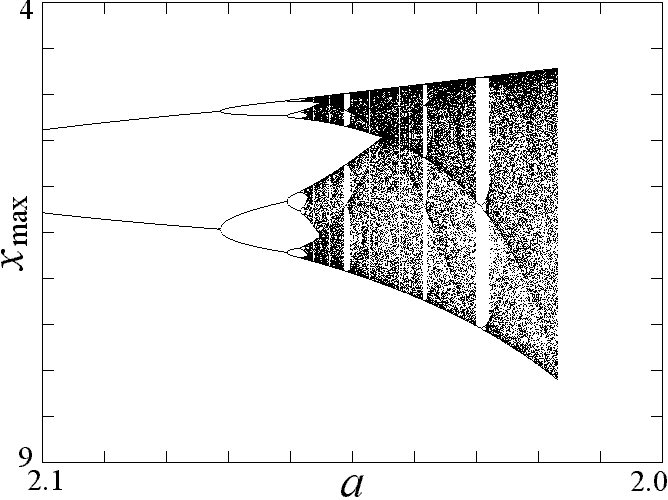
\includegraphics[width=8.4cm]{Figures/bifurcation.jpg}    % The printed column width is 8.4 cm.
\caption{Bifurcation: Plot of local maxima of $x$ with damping $a$ decreasing} 
\label{fig:bifurcation}
\end{center}
\end{figure}


\subsection{Tables}
Tables must be centered and have a caption above them, numbered with
Arabic numerals. See table~\ref{tab10} for an example.

\begin{table}[h]
\centering
\begin{tabular}{lllllllllll}
\hline
$b/r$                          & 0.1  & 0.5  & 1    & 5    & 10   & 25   & 50   & 100  & 200  & 500  \\
\hline
$AGap^{\ast}$ (\%)    & 0.74 & 0.37 & 0.14 & 0.04 & 0.01 & 0.00 & 0.01 & 0.03 & 0.00 & 0.00 \\
$AGapH^{\ast}$ (\%) & 5.19 & 3.73 & 2.95 & 2.87 & 2.27 & 1.45 & 1.17 & 0.83 & 0.84 & 0.64 \\
\textit{ACPU times (s)}                 & 0.29 & 0.26 & 0.17 & 0.13 & 0.11 & 0.09 & 0.12 & 0.09 & 0.08 & 0.09 \\
\textit{ACPUH times (s)}               & 0.03 & 0.03 & 0.03 & 0.03 & 0.03 & 0.02 & 0.02 & 0.02 & 0.02 & 0.02 \\
\hline    
\end{tabular}
\caption{Performances of HGA and the proposed heuristic.}
\label{tab10}
\end{table}
\section{Conclusions et perspectives}\label{sec:conclusion}
In this study, we examined...

\section{Plagiat}
Je tiens à vous informer que tous les travaux que vous allez nous remettre seront soumis à une vérification de plagiat à l'aide d'un logiciel spécialisé. Il est essentiel que votre travail soit original et reflète vos propres efforts et apprentissages. Toute tentative de plagiat sera rigoureusement sanctionnée, conformément aux règlements de notre établissement. Je vous encourage donc à vous assurer que vos rapports sont authentiques et à bien citer vos sources lorsque cela est nécessaire.

% \printbibliography

\bibliography{references2}
\end{document}